\section{Auswertung}
\label{sec:Auswertung}
Für die Untersuchung der verschiedenen $\gamma$-Spektren werden die Kanäle des ``ADC'' auf die entsprechenden Energien kalibriert. Desweiteren wird die Effizienz des Detektors exemplarisch an dem EU-Spektrum berechnet und anschließend die Messwerte zur Bestimmung der aktivität der verwendeten Bariumquelle mit ihr bereinigt. Zuletzt wird anhand des Spektrums versucht auf die Zerfallsprodukte eines Minerals zu schließen und somit deren Zerfallskette zu bestimmen.
\subsection{Kalibrieren des Detektors anhand EU$^{152}$ Spektrums}
Zunächst wird die Kanalnummer auf die Energie anhand des Spektrums des EU$^{152}$ Strahlers kalibriert. Die Energie mit den entsprechenden Kanalnummern sind in Tabelle \ref{tab:CsSpekt} aufgeführt.
\begin{table}
  \centering
  \begin{tabular}{c | c c c c}
    \toprule
    Energie $E_{\gamma}$ / keV& Kanal & Emissionwahrscheinlichkeit / \% & Counts & Effizienz / \% \\	
    \hline
    121.78	& 403	& 28.6	& 3078 	& ---	\\
    244.70	& 803	& 7.6	& 485 	& \num{10.40 +- 0.1}	\\
    344.30	& 1128	& 26.5	& 1048	& \num{6.40 +- 0.1}	\\
    411.12	& 1345	& 2.2	& 79	& \num{5.80 +- 0.1}	\\
    443.96	& 1452	& 3.1	& 112 	& \num{5.90 +- 0.1}	\\
    778.90	& 2544	& 12.9	& 193	& \num{2.44 +- 0.04}	\\
    867.37	& 2832	& 4.2	& 61	& \num{2.36 +- 0.03}	\\
    964.08	& 3147	& 14.6	& 132	& \num{1.47 +- 0.02}	\\
    1085.90	& 3543	& 10.2	& 88	& \num{1.40 +- 0.02}	\\
    1112.10	& 3629	& 13.6	& 108	& \num{1.29 +- 0.02}	\\
    1408.00	& 4593	& 21.0 	& 134	& \num{1.04 +- 0.02}	\\
    \bottomrule
  \end{tabular}
  \caption{<+Caption text+>}
  \label{tab:CsSpekt}
\end{table} 
Um die Korrelation zwischen der Energie und der Kanalnummer zu bestimmen wird eine lineare Regression durch die Tupel aus Energie und Kanalnummer gelegt. Das Ergebniss ist in Abbildung \ref{fig:RegCs} zu sehen. 
\begin{figure}
  \centering
  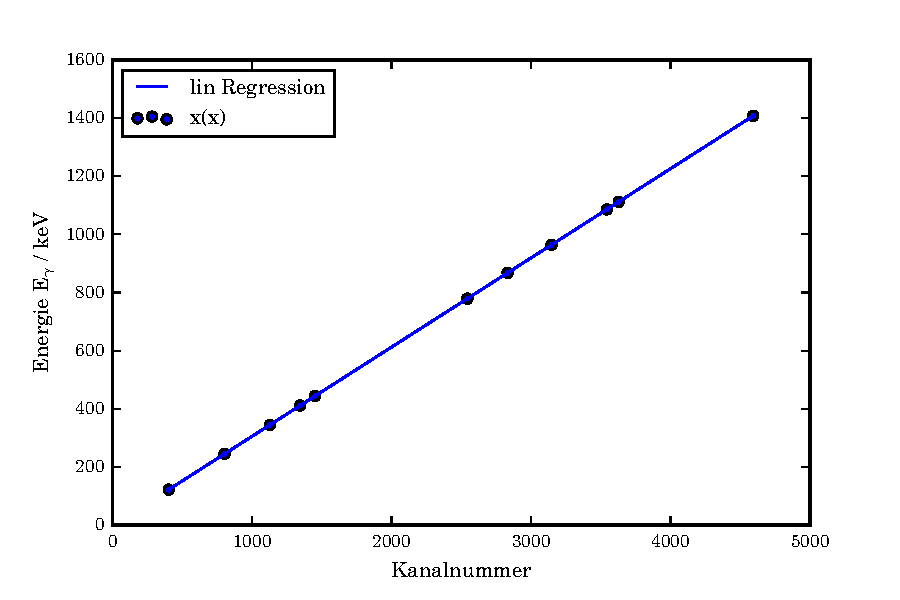
\includegraphics[width=\textwidth]{./build/CsReg.pdf}
  \caption{<+caption text+>}
  \label{fig:RegCs}
\end{figure}
Aus der Regression ergibt sich eine Energiedifferenz zweier benachbarter Kanäle beträgt von 
\begin{equation}
  \Delta E = (\num{0.30697 +- 0.00003}) \, \text{eV}
  \label{eqn:Reg}
\end{equation}
Anhand der Energieskala werden die gemessenen Counts im weiteren in Abhängikeit der $\gamma$-Quanten Energie $E_{\gamma}$ dargestellt. Das für den Cs-Strahler aufgenommene Spektrum ist in Abbildung \ref{fig:SpekCs} zu sehen. 
\begin{figure}
  \centering
  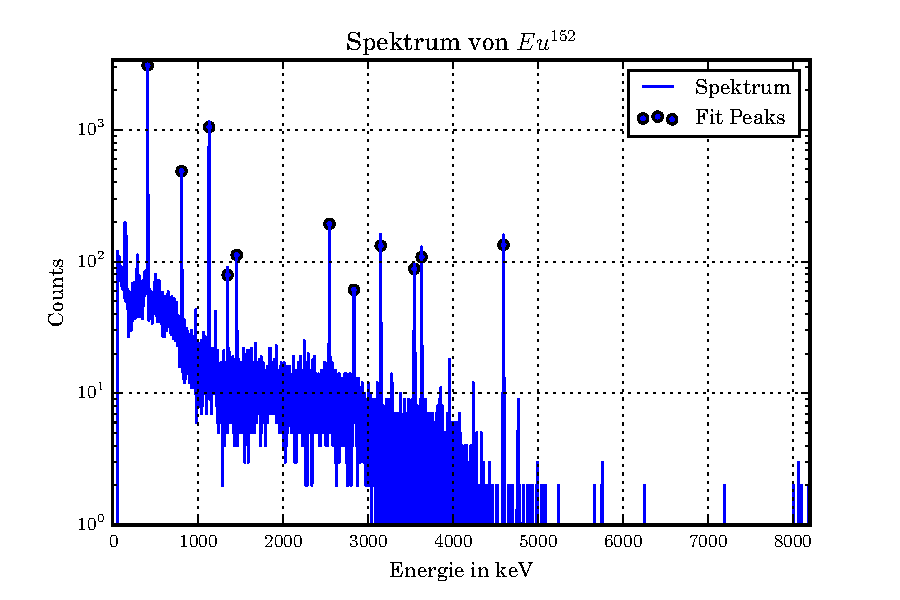
\includegraphics[width=\textwidth]{./build/SpektEu.pdf}
  \caption{<+caption text+>}
  \label{fig:SpekCs}
\end{figure}
Die Aktivität $A_\text{Eich}$ der verwendeten Europium Isotop betrug am 01.10.2000
\begin{equation}
  A_\text{Eich} = (\num{4130 +- 60}) \, \text{Bq} 
  \label{eqn:AktEu}
\end{equation}
und die Halbwertszeit
\begin{equation}
  \tau_{1/2} = (\num{4943 +- 5}) \, \text{Tage} 
  \label{eqn:halb}
\end{equation}
Anhand Formel \ref{eqn:??} lässt sich mittels der Zeitdifferenz zwischen der geeichten Aktivität und dem am Tag der Durchführung der Messung (09.01.2017) eine Aktivität von 
\begin{equation}
  A_\text{Durch} = (\num{1242 +- 35}) \, \text{Bq}
  \label{eqn:AktEEu}
\end{equation}
berechnen. Dem Versuchsaufbau wird ein Abstand $a$ zwischen Quelle und Detektor von 
\begin{equation}
  a = 8.8 \, \text{cm}
  \label{<++>}
\end{equation}
und ein Radius $r$ des Detektors von
\begin{equation}
  r = 2.25 \, \text{cm} 
  \label{<++>}
\end{equation}
gemessen. Aus diesen lässt sich durch einsetzen in Formel \ref{eqn:??} ein Raumwinkel $\Omega$ von 
\begin{equation}
  \Omega = 0.196 
  \label{eqn:Raum}
\end{equation}
berechnen. Aus dem Raumwinkel $\Omega$, der Wechselwirkungswahrscheinlickeit $W$, der Aktivität $A_\text{Durch}$ sowie die effektiv gemessene Zeit lässt sich nach Formel \ref{eqn:??} die Effizienz $Q$ berechnen. Die Ergebnisse in Abhängikeit der Energie sind in Tabelle \ref{tab:CsSpekt} aufgeführt. Um in erster Näherung die Effizienz in den folgenden Auswertungsteil \ref{sec:??} zur berücksichtigen wird die Effizenz in erster Näherung durch ein Potenzfunktion dargestellt. 
\begin{figure}
  \centering
  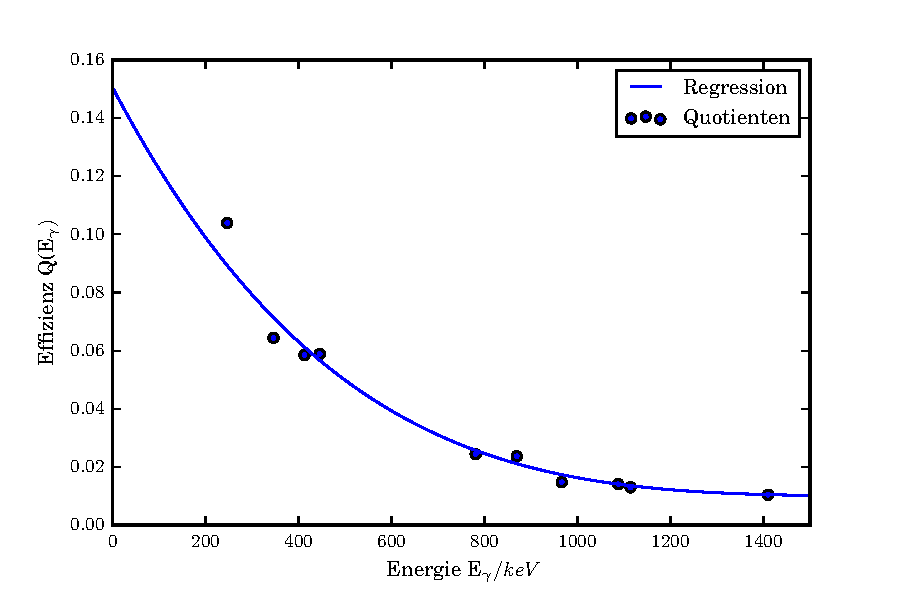
\includegraphics[width=\textwidth]{./build/Effizienz.pdf}
  \caption{<+caption text+>}
  \label{fig:<+label+>}
\end{figure}
Die ermittelte Potenzfunktion hatt die Form 
\begin{equation}
  Q(E_\gamma)= 1.2 \cdot 10^{-14} \left( x - 1850 \right)^4 + 0.01 \ .
  \label{eqn:QCs}
\end{equation}
